%==============Document Class==============
\documentclass[english,a4paper]{article}

%==============Packages==================
\usepackage[utf8]{inputenc}
\usepackage[T1]{fontenc}
\usepackage[english]{babel}
\usepackage[margin=2.5cm]{geometry}
\usepackage{hyperref}
\usepackage{graphicx}
\usepackage{listings}
\usepackage{xcolor}

\graphicspath{ {} }

%==============Code Formatting==================
\lstset{
    language=Java,
    basicstyle=\ttfamily\small,
    keywordstyle=\color{blue},
    stringstyle=\color{red},
    commentstyle=\color{green!60!black},
    numbers=left,
    numberstyle=\tiny,
    numbersep=5pt,
    frame=single,
    breaklines=true
}



%==============Title Configuration==================
\title{\Large MasterMind Game Implementation\\
\large Object-Oriented Programming Project}
\author{Erkin Tunc Boya}
\date{April 2025}

%==============Document Start==================
\begin{document}
\maketitle

%==============Introduction==================
\section{Introduction}
This project implements a Java-based MasterMind game featuring multiple game modes, configurable difficulty settings, and an intelligent computer opponent. The implementation demonstrates object-oriented programming principles while providing an engaging gaming experience through its modular and extensible design.

%==============Game Overview==================
\section{Game Overview}
The core gameplay revolves around players attempting to guess a secret combination of colored pegs within a limited number of attempts. After each attempt, players receive feedback indicating:
\begin{itemize}
\item The number of pegs with correct color and position
\item The number of pegs with correct color but wrong position
\end{itemize}

The game offers three distinct modes:
\begin{itemize}
\item Single Player: Players compete against computer-generated combinations
\item Multiplayer: Supports player vs. player competition with tournament capabilities
\item AI Opponent: Players challenge an adaptive AI that employs sophisticated guessing strategies
\end{itemize}

%==============Technical Implementation==================
\section{Technical Implementation}
The implementation is structured around seven key classes that handle different aspects of the game:

%==============Core Components==================
\subsection{Core Components}
\begin{itemize}
\item \texttt{MasterMind}: Serves as the main controller, managing game initialization and mode selection
\item \texttt{Game}: Handles game session management, including turn progression and scoring
\item \texttt{Board}: Maintains game state, tracks attempts, and validates moves
\item \texttt{Player}: Provides base functionality for human players
\item \texttt{Combination}: Manages color combinations and validation logic
\item \texttt{Pion}: Represents individual pegs with color and position properties
\end{itemize}

%==============AI Implementation==================
\subsection{AI Implementation}
The \texttt{AutomaticPlayer} class implements an intelligent computer opponent using three progressive strategies:

1. \textbf{Initial Phase:} Employs random generation for early attempts to explore the solution space

2. \textbf{Pattern Recognition:} Analyzes previous attempts to identify:
\begin{itemize}
\item Successful color patterns
\item Position-specific color frequencies
\item Color combination effectiveness
\end{itemize}

3. \textbf{Intelligent Analysis:} Utilizes weighted scoring systems to:
\begin{itemize}
\item Track position-specific color success rates
\item Adapt strategy based on feedback
\item Optimize color selection for each position
\end{itemize}

%==============Configuration Options==================
\section{Configuration Options}
The game supports various customization options to adjust difficulty and gameplay experience:
\begin{itemize}
\item Number of pegs (3-5)
\item Available colors (4-8)
\item Maximum attempts (5-20)
\item Detailed feedback mode
\end{itemize}

%==============Future Enhancements==================
\section{Future Enhancements}
Potential improvements for future versions include:
\begin{itemize}
\item Enhanced AI strategies using machine learning
\item Graphical user interface implementation
\item Online multiplayer capabilities
\item Achievement and progression systems
\end{itemize}

%==============UML Diagram==================

\section{Class Diagram}

\begin{figure}[t]
\caption{Master-Mind UML diagram}
	\centering
	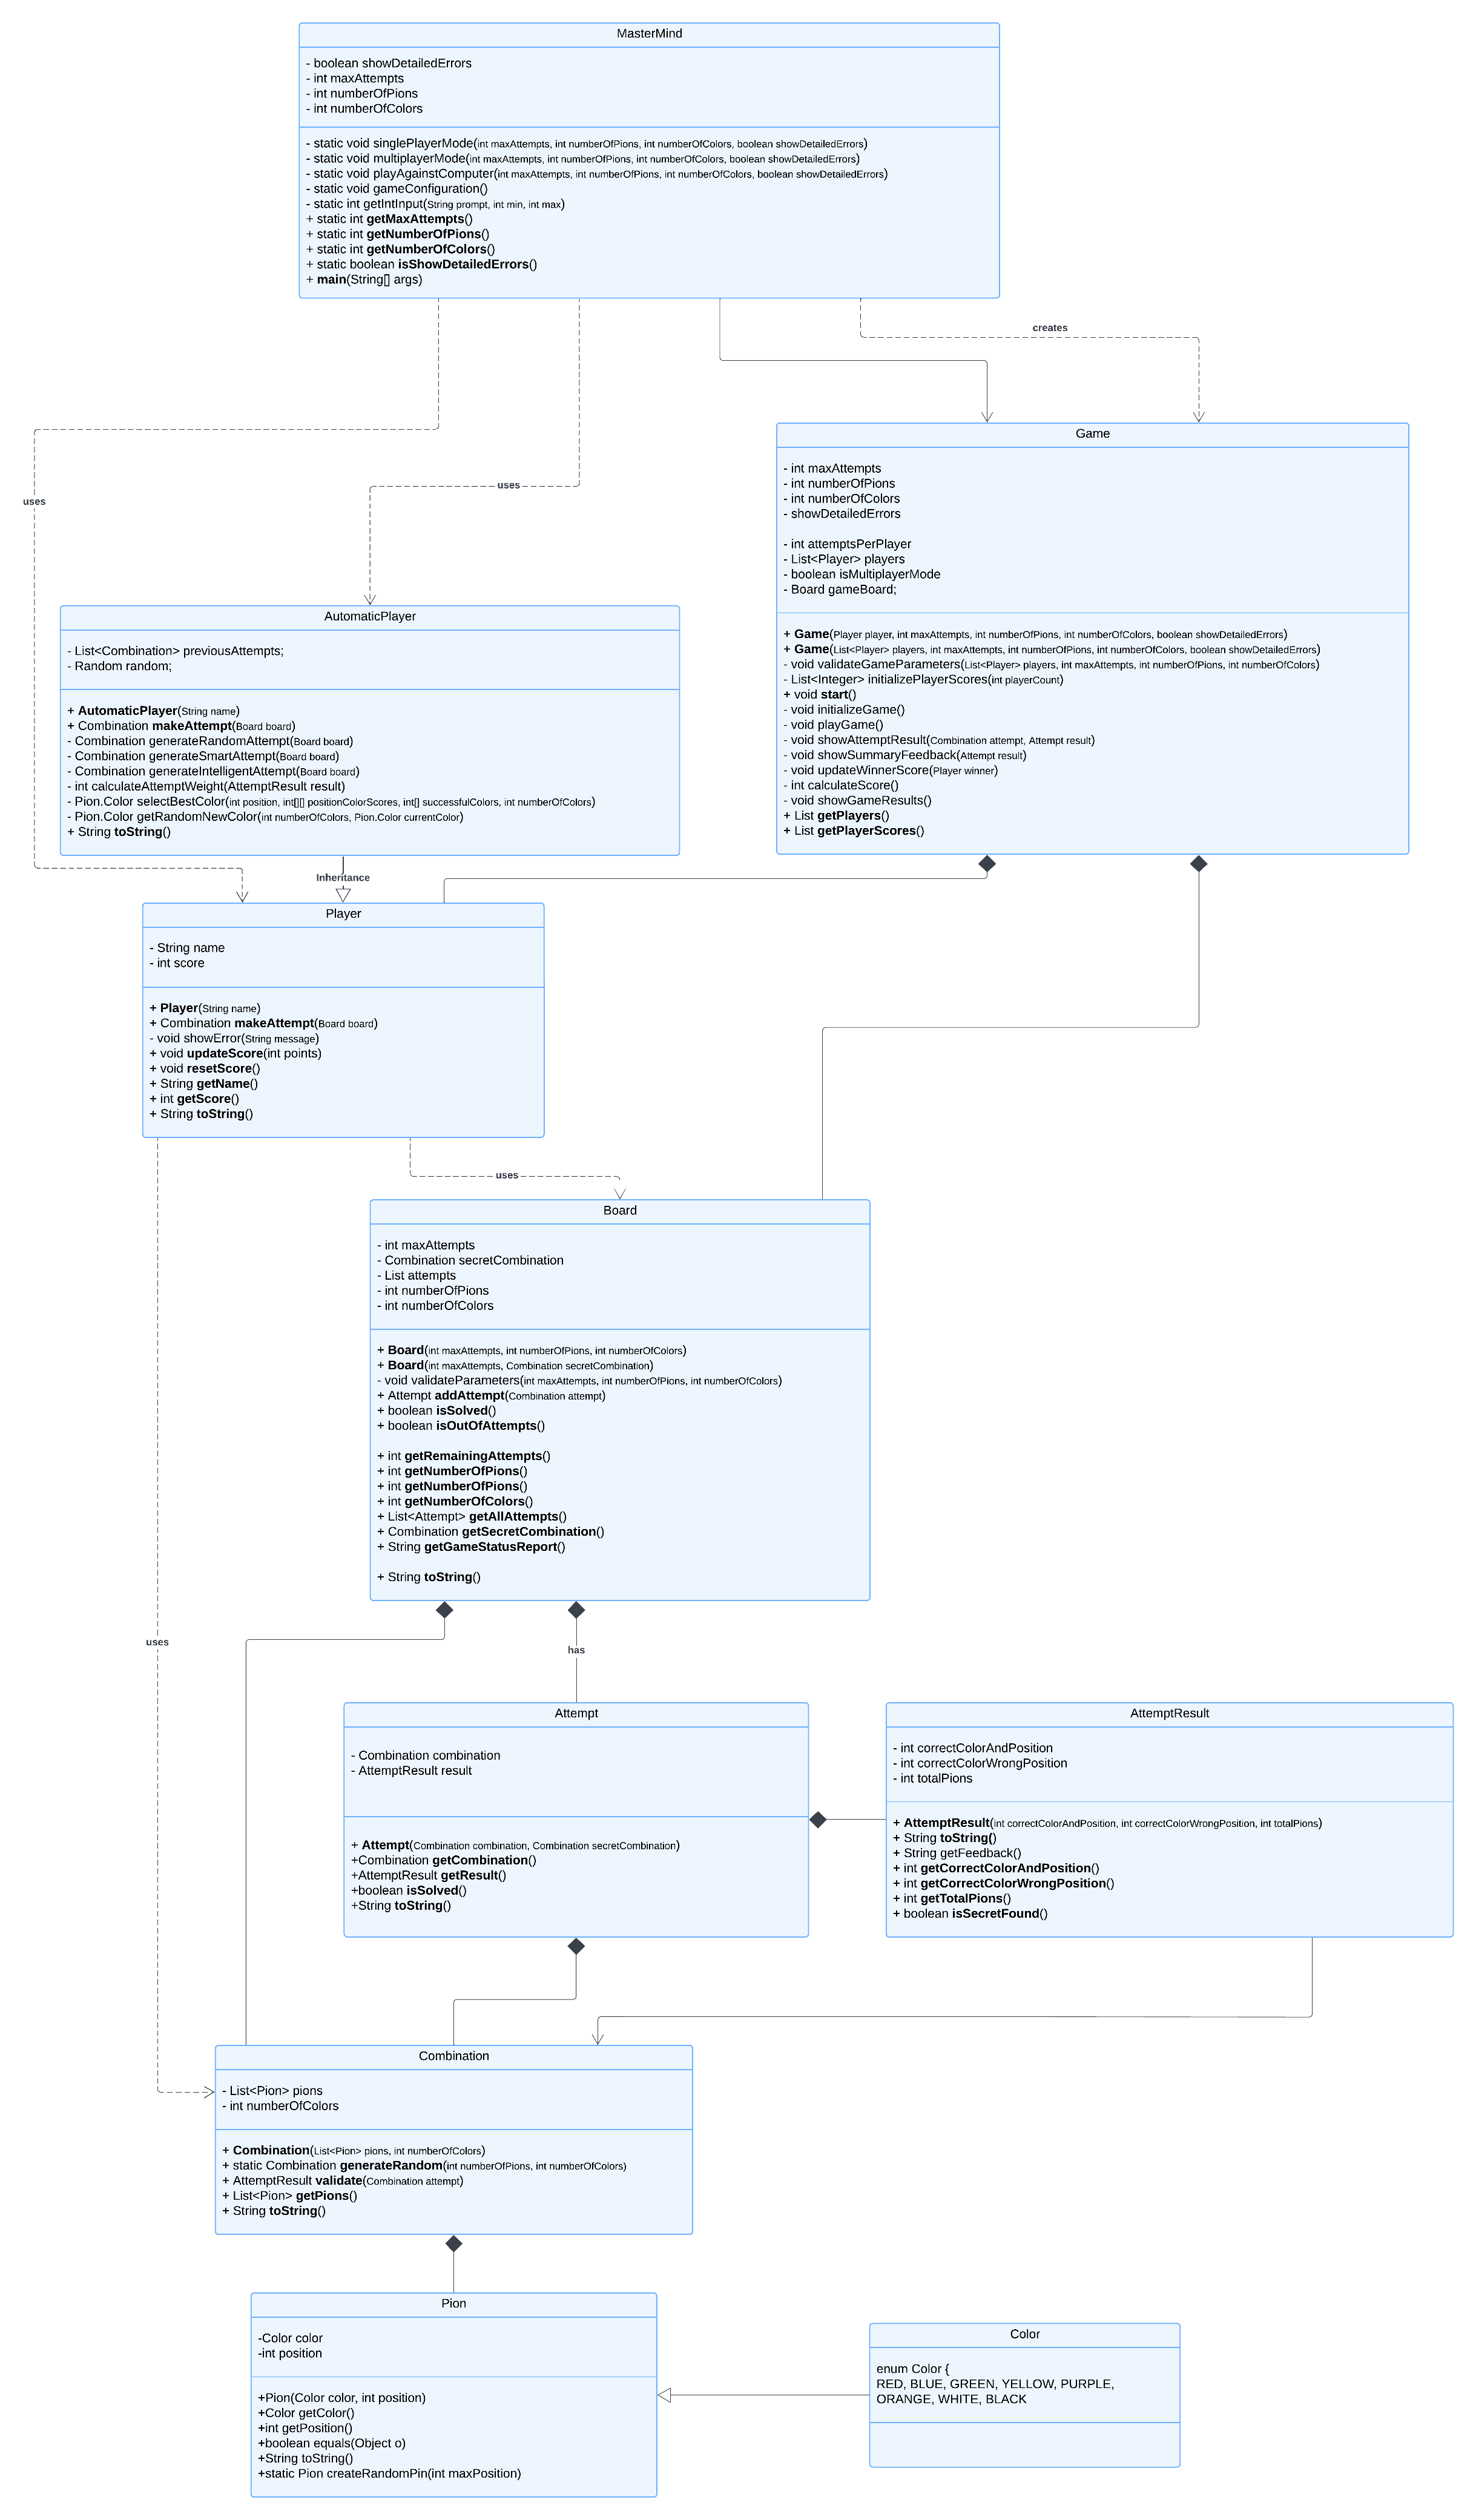
\includegraphics[scale=0.170]{MasterMind.png}
\end{figure}


\end{document}